\chapter{Convolution}
\label{ch:lesson10}

Convolution is the core operation behind blurring, sharpening, and edge detection --- and it's also the operation at the heart of a convolutional neural network's convolution layers (a later chapter). This chapter builds it from scratch, clarifies a common point of confusion (convolution vs.\ correlation), and shows a few classic filters.

\section{1D convolution}

Before tackling 2D images, start with the simpler problem of convolving two 1D arrays. For a signal $I$ and a kernel $K$, the discrete convolution is
\begin{equation}
(I * K)(x) = \sum_{i} K(i)\, I(x - i).
\end{equation}
Concretely: \textbf{flip} the kernel end-to-end, \textbf{slide} it along the signal one position at a time, and at each position take the dot product between the flipped kernel and the overlapping chunk of signal.

\begin{lstlisting}
def convolve1d(signal, kernel):
    ksize, pad = len(kernel), len(kernel) // 2
    padded = np.pad(signal, pad, mode='constant')
    flipped = kernel[::-1]
    out = np.zeros_like(signal, dtype=np.float64)
    for n in range(len(signal)):
        out[n] = np.dot(padded[n:n + ksize], flipped)
    return out
\end{lstlisting}

With signal $[1,2,3,4,5,4,3,2,1]$ and a 3-tap derivative kernel $[-1,0,1]$ (scaled by $0.5$), the from-scratch result matches \code{np.convolve} exactly (Figure~\ref{fig:l10-1}).

\begin{figure}[h]
\centering
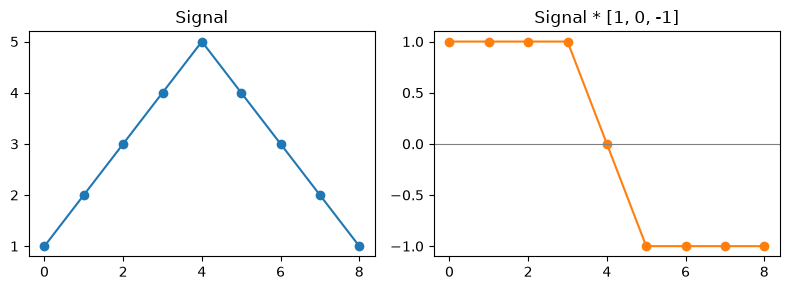
\includegraphics[width=0.7\textwidth]{figures/lesson10_fig01.png}
\caption{A ramp-up-then-down signal and its convolution with a derivative kernel: positive while rising, zero at the peak, negative while falling.}
\label{fig:l10-1}
\end{figure}

\section{2D convolution}

The 2D version (what actually gets used on images) is the same flip-and-slide idea, over two axes:
\begin{equation}
(I * K)(x, y) = \sum_{i}\sum_{j} K(i, j)\, I(x - i,\, y - j).
\end{equation}
Just as in 1D, the key detail is the \emph{minus} signs: the kernel is flipped ($180^\circ$ rotated) before it's slid across the image, which matters whenever the kernel is not symmetric. \textbf{Correlation} is the same idea without the flip:
\begin{equation}
(I \star K)(x, y) = \sum_{i}\sum_{j} K(i, j)\, I(x + i,\, y + j).
\end{equation}
In practice, most image-processing libraries --- including OpenCV's \code{cv2.filter2D} --- actually implement \emph{correlation}, not convolution, even though people casually call it ``convolving with a kernel.'' For symmetric kernels (box blur, Gaussian) the two are identical, so the distinction rarely matters in practice. But it is worth knowing the difference exists.

\subsection*{Convolution from scratch}

Flip the kernel both horizontally and vertically, pad the image so the kernel never runs off the edge, then at every position multiply the flipped kernel elementwise by the pixels underneath it and sum. For speed, the implementation below loops over the kernel's (few) entries rather than the image's (many) pixels, shifting and accumulating the whole padded image at once for each kernel weight.

\begin{lstlisting}
def convolve2d(image, kernel, border=cv2.BORDER_REFLECT101):
    kh, kw = kernel.shape
    ph, pw = kh // 2, kw // 2
    flipped = kernel[::-1, ::-1]
    padded = cv2.copyMakeBorder(image, ph, ph, pw, pw, border)
    out = np.zeros(image.shape, dtype=np.float64)
    for i in range(kh):
        for j in range(kw):
            out += flipped[i, j] * padded[i:i+image.shape[0], j:j+image.shape[1]]
    return out
\end{lstlisting}

Checked against \code{cv2.filter2D} fed the pre-flipped kernel (since \code{filter2D} computes correlation): max absolute difference is exactly $0.0$. Figure~\ref{fig:l10-2} also shows what correlation (no flip) gives instead.

\begin{figure}[h]
\centering
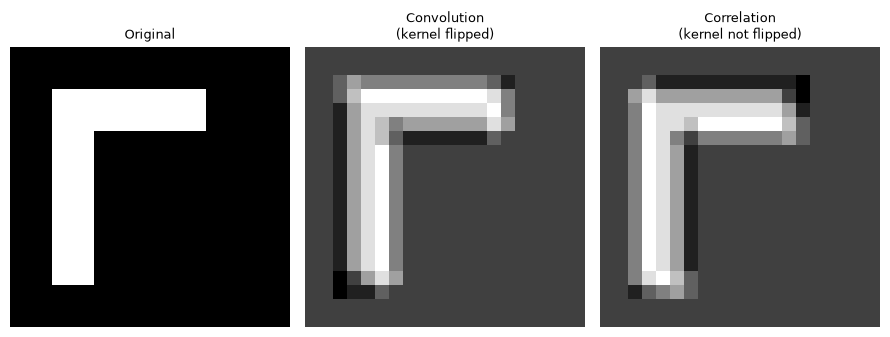
\includegraphics[width=0.85\textwidth]{figures/lesson10_fig02.png}
\caption{An asymmetric test shape, its convolution (kernel flipped), and its correlation (kernel not flipped) with the same asymmetric kernel --- visibly different results.}
\label{fig:l10-2}
\end{figure}

\section{Boundary handling}

Near the edges, the kernel hangs off the image. \code{convolve2d} uses \code{cv2.copyMakeBorder} to pad first; the padding mode changes the result at the border. Common choices: constant (zero) padding, replicate (extend the edge pixel), and reflect (mirror across the edge; \code{REFLECT101} avoids duplicating the edge pixel itself).

\section{Classic filters as kernels}

Once convolution works, most filters are just ``pick a kernel'':
\begin{itemize}
  \item \textbf{Box blur}: every neighbor weighted equally --- averages out noise but blurs edges.
  \item \textbf{Gaussian blur}: neighbors weighted by a bell curve --- smoother falloff, less ``boxy'' artifacting than a box blur.
  \item \textbf{Sharpen}: boosts the center pixel relative to its neighbors.
  \item \textbf{Sobel (edge detection)}: an asymmetric kernel that responds strongly to intensity changes in one direction --- a case where the convolution-vs-correlation flip actually matters, since the kernel is asymmetric (results in a sign flip).
\end{itemize}
Figure~\ref{fig:l10-3} shows all four filters applied to the same noisy photo.

\begin{figure}[h]
\centering
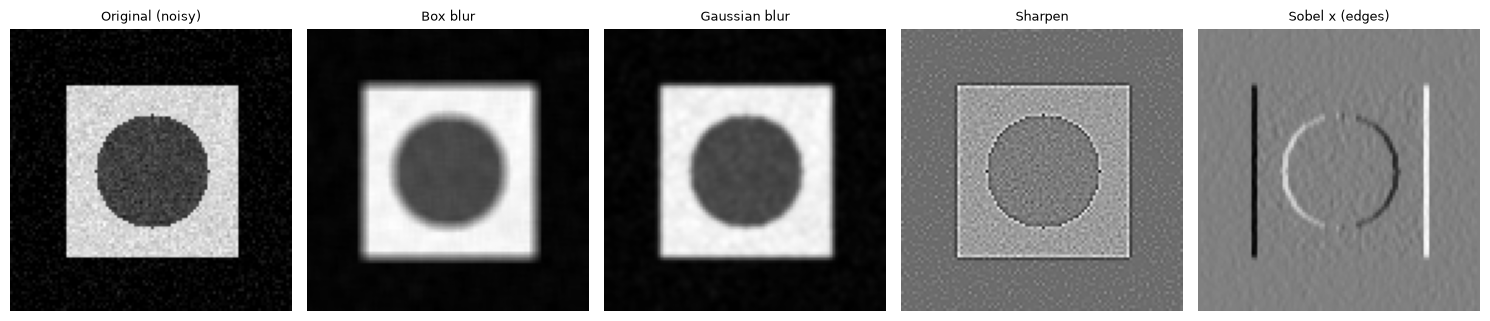
\includegraphics[width=0.95\textwidth]{figures/lesson10_fig03.png}
\caption{A noisy synthetic photo, then box blur, Gaussian blur, sharpen, and Sobel-$x$ edge detection, all implemented with the same \code{convolve2d} function above.}
\label{fig:l10-3}
\end{figure}

\subsection*{Separable kernels: a speed trick}

The Gaussian kernel above is \textbf{separable}: it can be written as the outer product of two 1D kernels, $K=k_x\,k_y^\top$. That means convolving with the full $n\times n$ kernel is equivalent to convolving with a $1\times n$ kernel, then an $n\times1$ kernel --- turning $O(n^2)$ work per pixel into $O(2n)$.

\begin{lstlisting}
separable_result = convolve2d(convolve2d(photo, k1d.reshape(1, -1)), k1d.reshape(-1, 1))
full_result = convolve2d(photo, gaussian)
# separable_result == full_result, to floating-point precision
\end{lstlisting}

\subsection*{Exercises}
\begin{enumerate}
  \item Verify that the box kernel is also separable, by writing it as an outer product of two 1D uniform kernels.
  \item \code{sobel\_x} above is not symmetric. Compute both the convolution and correlation of the noisy photo with it, and describe how the two outputs differ (hint: think about which direction of intensity change each responds to).
  \item Time \code{convolve2d} against \code{cv2.filter2D} on a $300\times300$ image with a $15\times15$ Gaussian kernel using \code{\%timeit}. Then time the separable two-pass version against the full 2D version. How much faster is each speedup?
\end{enumerate}

\vfill
\fullcode{lesson10}{lesson10_convolution}
